% Paper A application-context routing schematic.
% Direct, hand-authored TikZ; no generated or raster content.
% Palette provenance: submissions/frame-a-eswa/figures-r/make_figures_frame_a.R
% Build provenance: `make` in this directory (pdflatex + pdfjam + pdftoppm, CPU-only).
% Sizing rationale: standalone canvas 192.4mm wide so the figure scales down to
% ESWA preprint `\linewidth` = 390pt at ratio 0.712. Every text class is set to
% >=9.4pt nominal so its rendered size stays near 7pt at 390pt inclusion.
\documentclass[10pt,border=0.8pt]{standalone}
\usepackage[T1]{fontenc}
\usepackage{lmodern}
\usepackage{tikz}
\usetikzlibrary{arrows.meta,calc,positioning,shapes.geometric}

\newcommand{\FAfont}{\sffamily}

% Existing Frame-A multi-hue palette.
\definecolor{FAblue}{HTML}{2A78D6}
\definecolor{FAaqua}{HTML}{1BAF7A}
\definecolor{FAorange}{HTML}{EB6834}
\definecolor{FAviolet}{HTML}{4A3AA7}
\definecolor{FAred}{HTML}{E34948}
\definecolor{FAyellow}{HTML}{EDA100}
\definecolor{FAink}{HTML}{0B0B0B}
\definecolor{FAinktwo}{HTML}{333333}
\definecolor{FAtick}{HTML}{666666}
\definecolor{FAgrid}{HTML}{E1E0D9}
\definecolor{FAsurface}{HTML}{FCFCFB}

\begin{document}
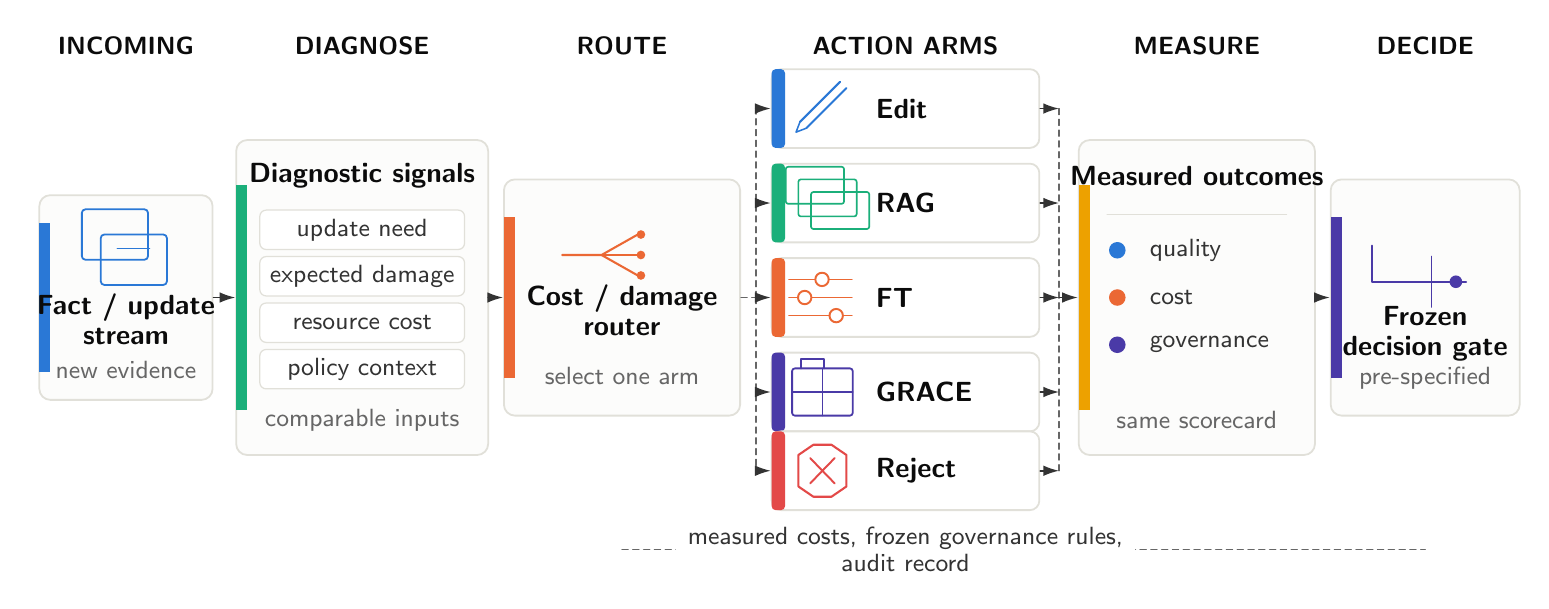
\begin{tikzpicture}[
  x=1mm,y=1mm,
  font=\FAfont\fontsize{9.4}{10.6}\selectfont,
  line cap=round,line join=round,
  >={Latex[length=2.0mm,width=1.35mm]},
  flow/.style={draw=FAinktwo,line width=0.55pt,-{Latex[length=2.0mm,width=1.35mm]}},
  control/.style={draw=FAtick,line width=0.5pt,dash pattern=on 2.2pt off 1.7pt},
  stage/.style={draw=FAgrid,line width=0.65pt,rounded corners=1.4mm,fill=FAsurface,
    align=center,inner sep=0pt},
  card/.style={draw=FAgrid,line width=0.65pt,rounded corners=1.2mm,fill=white,
    minimum width=34mm,minimum height=10mm,inner sep=0pt},
  chip/.style={draw=FAgrid,line width=0.45pt,rounded corners=0.8mm,fill=white,
    minimum width=26mm,minimum height=5.0mm,anchor=center,inner sep=0pt,
    font=\FAfont\fontsize{9.0}{10.2}\selectfont,text=FAinktwo},
  heading/.style={font=\FAfont\bfseries\fontsize{9.4}{10.6}\selectfont,
    text=FAink,align=center},
  body/.style={font=\FAfont\fontsize{9.0}{10.2}\selectfont,text=FAinktwo},
  strong/.style={font=\FAfont\bfseries\fontsize{9.6}{10.8}\selectfont,text=FAink},
  audit/.style={font=\FAfont\fontsize{8.8}{10.0}\selectfont,text=FAinktwo,
    align=center,fill=white,inner xsep=1.5mm}
]

% Column headings keep the reading order explicit at journal page width.
\node[heading] at (11,32) {INCOMING};
\node[heading] at (41,32) {DIAGNOSE};
\node[heading] at (74,32) {ROUTE};
\node[heading] at (110,32) {ACTION ARMS};
\node[heading] at (147,32) {MEASURE};
\node[heading] at (176,32) {DECIDE};

% 1. Incoming fact/update stream.
\node[stage,minimum width=22mm,minimum height=26mm] (incoming) at (11,0) {};
\fill[FAblue] ([xshift=-11mm,yshift=9.4mm]incoming.center)
  rectangle ([xshift=-9.6mm,yshift=-9.4mm]incoming.center);
% Two compact update cards (outline glyph).
\draw[FAblue,line width=0.65pt,rounded corners=0.45mm]
  ([xshift=-5.6mm,yshift=4.8mm]incoming.center) rectangle ++(8.4mm,6.4mm);
\draw[FAblue,line width=0.65pt,rounded corners=0.45mm]
  ([xshift=-3.2mm,yshift=1.6mm]incoming.center) rectangle ++(8.4mm,6.4mm);
\draw[FAblue,line width=0.5pt]
  ([xshift=-1.1mm,yshift=6.2mm]incoming.center) -- ++(4.1mm,0);
\node[strong,align=center] at ([yshift=-2.8mm]incoming.center) {Fact / update\\stream};
\node[body,align=center,text=FAtick] at ([yshift=-9.2mm]incoming.center)
  {new evidence};

% 2. Diagnostic signals.
\node[stage,minimum width=32mm,minimum height=40mm] (diag) at (41,0) {};
\fill[FAaqua] ([xshift=-16mm,yshift=14.3mm]diag.center)
  rectangle ([xshift=-14.6mm,yshift=-14.3mm]diag.center);
\node[strong] at ([yshift=15.5mm]diag.center) {Diagnostic signals};
\node[chip] at ([yshift=8.6mm]diag.center) {update need};
\node[chip] at ([yshift=2.7mm]diag.center) {expected damage};
\node[chip] at ([yshift=-3.2mm]diag.center) {resource cost};
\node[chip] at ([yshift=-9.1mm]diag.center) {policy context};
\node[body,align=center,text=FAtick] at ([yshift=-15.6mm]diag.center)
  {comparable inputs};

% 3. Cost/damage router.
\node[stage,minimum width=30mm,minimum height=30mm] (router) at (74,0) {};
\fill[FAorange] ([xshift=-15mm,yshift=10.2mm]router.center)
  rectangle ([xshift=-13.6mm,yshift=-10.2mm]router.center);
% Outline routing glyph: one inlet, three candidate branches.
\draw[FAorange,line width=0.75pt] ([xshift=-7.6mm,yshift=5.4mm]router.center)
  -- ([xshift=-2.6mm,yshift=5.4mm]router.center)
  -- ([xshift=2.0mm,yshift=8.0mm]router.center);
\draw[FAorange,line width=0.75pt] ([xshift=-2.6mm,yshift=5.4mm]router.center)
  -- ([xshift=2.0mm,yshift=5.4mm]router.center);
\draw[FAorange,line width=0.75pt] ([xshift=-2.6mm,yshift=5.4mm]router.center)
  -- ([xshift=2.0mm,yshift=2.8mm]router.center);
\foreach \yy in {8.0,5.4,2.8}{\fill[FAorange] ([xshift=2.4mm,yshift=\yy mm]router.center) circle (0.55mm);}
\node[strong,align=center] at ([yshift=-1.6mm]router.center) {Cost / damage\\router};
\node[body,align=center,text=FAtick] at ([yshift=-10.0mm]router.center)
  {select one arm};

% 4. Five action cards: hue + label + unique outline glyph provide redundant identity.
\foreach \name/\yy/\col in {edit/24/FAblue,rag/12/FAaqua,ft/0/FAorange,grace/-12/FAviolet,reject/-22/FAred}{
  \node[card] (\name) at (110,\yy) {};
  \fill[\col,rounded corners=0.5mm]
    ([xshift=-17mm,yshift=5mm]\name.center) rectangle
    ([xshift=-15.3mm,yshift=-5mm]\name.center);
}
% Pencil glyph.
\draw[FAblue,line width=0.75pt]
  ([xshift=-13.4mm,yshift=-1.7mm]edit.center) -- ([xshift=-8.3mm,yshift=3.4mm]edit.center);
\draw[FAblue,line width=0.75pt]
  ([xshift=-12.6mm,yshift=-2.5mm]edit.center) -- ([xshift=-7.5mm,yshift=2.6mm]edit.center);
\draw[FAblue,line width=0.55pt]
  ([xshift=-13.4mm,yshift=-1.7mm]edit.center) -- ([xshift=-13.9mm,yshift=-3.0mm]edit.center)
  -- ([xshift=-12.6mm,yshift=-2.5mm]edit.center);
\node[strong,anchor=west] at ([xshift=-5mm]edit.center) {Edit};
% Retrieval-stack glyph.
\foreach \dx/\dy in {-1.6/1.6,0/0,1.6/-1.6}{
  \draw[FAaqua,line width=0.6pt,rounded corners=0.3mm]
    ([xshift=-13.6mm+\dx mm,yshift=-1.7mm+\dy mm]rag.center) rectangle ++(7.4mm,4.7mm);
}
\node[strong,anchor=west] at ([xshift=-5mm]rag.center) {RAG};
% Fine-tuning sliders glyph.
\foreach \dy/\cx in {2.3/-10.6,0/-12.8,-2.3/-8.8}{
  \draw[FAorange,line width=0.55pt]
    ([xshift=-14.8mm,yshift=\dy mm]ft.center) -- ([xshift=-6.8mm,yshift=\dy mm]ft.center);
  \draw[FAorange,line width=0.7pt,fill=white]
    ([xshift=\cx mm,yshift=\dy mm]ft.center) circle (0.85mm);
}
\node[strong,anchor=west] at ([xshift=-5mm]ft.center) {FT};
% GRACE codebook glyph (tabbed grid).
\draw[FAviolet,line width=0.65pt,rounded corners=0.35mm]
  ([xshift=-14.4mm,yshift=-3.0mm]grace.center) rectangle ++(7.7mm,6.0mm);
\draw[FAviolet,line width=0.55pt]
  ([xshift=-10.55mm,yshift=-3.0mm]grace.center) -- ([xshift=-10.55mm,yshift=3.0mm]grace.center)
  ([xshift=-14.4mm,yshift=0mm]grace.center) -- ([xshift=-6.7mm,yshift=0mm]grace.center);
\draw[FAviolet,line width=0.65pt]
  ([xshift=-13.3mm,yshift=3.0mm]grace.center) -- ++(0,1.2mm) -- ++(3.0mm,0) -- ++(0,-1.2mm);
\node[strong,anchor=west] at ([xshift=-5mm]grace.center) {GRACE};
% Stop badge glyph.
\draw[FAred,line width=0.75pt]
  ([xshift=-13.6mm,yshift=2.0mm]reject.center) -- ([xshift=-11.7mm,yshift=3.3mm]reject.center)
  -- ([xshift=-9.4mm,yshift=3.3mm]reject.center) -- ([xshift=-7.5mm,yshift=2.0mm]reject.center)
  -- ([xshift=-7.5mm,yshift=-2.0mm]reject.center) -- ([xshift=-9.4mm,yshift=-3.3mm]reject.center)
  -- ([xshift=-11.7mm,yshift=-3.3mm]reject.center) -- ([xshift=-13.6mm,yshift=-2.0mm]reject.center) -- cycle;
\draw[FAred,line width=0.7pt]
  ([xshift=-12.1mm,yshift=1.6mm]reject.center) -- ([xshift=-9.0mm,yshift=-1.6mm]reject.center)
  ([xshift=-9.0mm,yshift=1.6mm]reject.center) -- ([xshift=-12.1mm,yshift=-1.6mm]reject.center);
\node[strong,anchor=west] at ([xshift=-5mm]reject.center) {Reject};

% 5. Measured outcomes: neutral text, colored marks only.
\node[stage,minimum width=30mm,minimum height=40mm] (measure) at (147,0) {};
\fill[FAyellow] ([xshift=-15mm,yshift=14.3mm]measure.center)
  rectangle ([xshift=-13.6mm,yshift=-14.3mm]measure.center);
\node[strong] at ([yshift=15.5mm]measure.center) {Measured outcomes};
\draw[FAgrid,line width=0.45pt] ([xshift=-11.4mm,yshift=10.5mm]measure.center) -- ([xshift=11.4mm,yshift=10.5mm]measure.center);
\fill[FAblue] ([xshift=-10.1mm,yshift=6.0mm]measure.center) circle (1.05mm);
\node[body,anchor=west] at ([xshift=-7.2mm,yshift=6.0mm]measure.center) {quality};
\fill[FAorange] ([xshift=-10.1mm,yshift=0mm]measure.center) circle (1.05mm);
\node[body,anchor=west] at ([xshift=-7.2mm,yshift=0mm]measure.center) {cost};
\fill[FAviolet] ([xshift=-10.1mm,yshift=-6.0mm]measure.center) circle (1.05mm);
\node[body,anchor=west] at ([xshift=-7.2mm,yshift=-6.0mm]measure.center) {governance};
\node[body,align=center,text=FAtick] at ([yshift=-15.6mm]measure.center)
  {same scorecard};

% 6. Frozen decision gate.
\node[stage,minimum width=24mm,minimum height=30mm] (gate) at (176,0) {};
\fill[FAviolet] ([xshift=-12mm,yshift=10.2mm]gate.center)
  rectangle ([xshift=-10.6mm,yshift=-10.2mm]gate.center);
% Gate/threshold glyph.
\draw[FAviolet,line width=0.7pt]
  ([xshift=-6.7mm,yshift=6.6mm]gate.center) -- ([xshift=-6.7mm,yshift=2.0mm]gate.center)
  -- ([xshift=5.2mm,yshift=2.0mm]gate.center);
\draw[FAviolet,line width=0.7pt]
  ([xshift=0.8mm,yshift=-1.2mm]gate.center) -- ([xshift=0.8mm,yshift=5.2mm]gate.center);
\fill[FAviolet] ([xshift=3.9mm,yshift=2.0mm]gate.center) circle (0.8mm);
\node[strong,align=center] at ([yshift=-4.6mm]gate.center) {Frozen\\decision gate};
\node[body,align=center,text=FAtick] at ([yshift=-10.2mm]gate.center)
  {pre-specified};

% Main left-to-right flow.
\draw[flow] (incoming.east) -- (diag.west);
\draw[flow] (diag.east) -- (router.west);
\draw[flow] (measure.east) -- (gate.west);

% Dashed control buses make selection and aggregation explicit without implying
% empirical superiority of any arm.
\coordinate (branch) at (91,0);
\draw[control] (router.east) -- (branch);
\draw[control] (branch) -- (91,24);
\draw[control] (branch) -- (91,-22);
\foreach \arm in {edit,rag,ft,grace,reject}{
  \draw[flow] (91,0 |- \arm.center) -- (\arm.west);
}
\coordinate (merge) at (129.5,0);
\draw[control] (129.5,24) -- (129.5,-22);
\foreach \arm in {edit,rag,ft,grace,reject}{
  \draw[flow] (\arm.east) -- (129.5,0 |- \arm.center);
}
\draw[flow] (merge) -- (measure.west);

% A separate audit/control lane stays outside the data path.
\draw[control] ([yshift=-32mm]router.center) -- ([yshift=-32mm]gate.center);
\node[audit] at (110,-32)
  {measured costs, frozen governance rules,\\audit record};

\end{tikzpicture}
\end{document}